%%%%%%%%%%%%
%
% $Autor: Wings $
% $Datum: 2019-03-05 08:03:15Z $
% $Pfad: TemplateSensor $
% $Version: 4250 $
% !TeX spellcheck = en_GB/de_DE
% !TeX encoding = utf8
% !TeX root = filename 
% !TeX TXS-program:bibliography = txs:///biber
%
%%%%%%%%%%%%
\documentclass{article}
% Structure
\section{\textcolor{red}{Sensor Lichtschranke}}

Introduction
\Mynote{cite books, applications, board}

\subsection{General}

\STANDARD{Funktionsprinzip}
{ 
	\textbf{Grundsätzlich:} Wandlung einer \textbf{nicht elektrischen Eingangsgröße} in ein \textbf{elektrisches Ausgangssignal}. \cite{Hering:2023}
	\begin{center}
		\begin{figure}
			\usetikzlibrary{arrows.meta, positioning}
			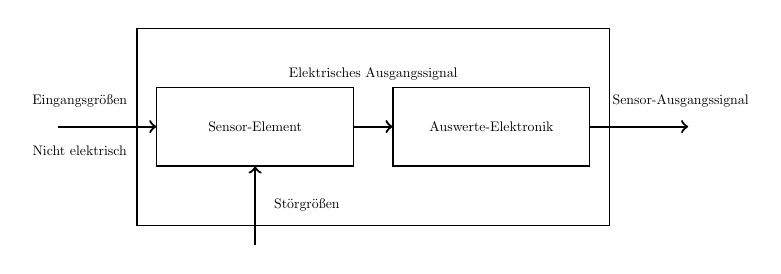
\begin{tikzpicture}[
				scale=0.5,
				transform shape,
				block/.style={draw, rectangle, minimum width=5cm, minimum height=2cm, align=center},
				outer/.style={draw, rectangle, minimum width=12cm, minimum height=5cm},
				arrow/.style={->, thick}
				]
				
				% Outer box
				\node[outer] (system) {};
				
				% Inner blocks
				\node[block] (sensor) at (-3,0) {Sensor-Element};
				\node[block] (eval) at (3,0) {Auswerte-Elektronik};
				
				% Input arrow
				\draw[arrow] (-8,0) -- (sensor.west)
				node[midway, above, xshift=-20pt, yshift=10pt] {Eingangsgrößen}
				node[midway, below, xshift=-20pt, yshift=-10pt] {Nicht elektrisch};
				
				% Between blocks
				\draw[arrow] (sensor.east) -- (eval.west)
				node[midway, above, yshift=30pt] {Elektrisches Ausgangssignal};
				
				% Output arrow
				\draw[arrow] (eval.east) -- (8,0)
				node[midway, above, xshift=30pt, yshift=10pt] {Sensor-Ausgangssignal};
				
				% Disturbance arrow
				\draw[arrow] (-3,-3) -- (sensor.south)
				node[midway, right, xshift=10pt] {Störgrößen};
				
			\end{tikzpicture}
			\caption{Wirkprinzip eines Sensorsystemes}
		\end{figure}	
	\end{center}
	\textbf{Achtung:} äußere Störgrößen können Einfluss nehmen und müssen daher berücksichtigt werden (z.B. Berücksichtigung der Temperaturabhängigkeit)
}

\section{Specific Sensor/Actor}



\section{Specification}

\begin{itemize}
  \item Cite the data sheet
  \item Extract te information from the data sheet
  \item Circuit Diagram
\end{itemize}

\section{Library}

\subsection{Description}

\subsection{Installation}

\begin{itemize}
    \item data types
    \item data structure
    \item data quantity
    \item data quality
\end{itemize}

\subsection{Functions}

\section{Example}

In this section, a simple example is described in detail, which demonstrates how the library supports the sensor/actor.


\subsection{Manual}

\subsection{Inside the Example}

\subsection{Code}

\subsection{Files}



\section{Calibration}

cite method

\section{Simple Code}


\section{Simple Application}



\section{Tests}

\subsection{Simple Function Test}

\subsection{Test all Functions}



\section{Further Readings}

